\begin{figure}[p]\centering
\caption[Construction and use of the layer-selection curve]{Construction and use of the layer-selection curve. A: each model supplies one split-sample AUC at each candidate index; their mean supplies one curve point. B: the saved means select index 22. C: re-estimated directions feed the four exploratory checks. The colored symbols in A are schematic outcome groups: blue denotes refused, orange denotes unsafe; their positions are not observed projections.}
% Symbolic construction of one layer-sweep point; no observed projections shown.
\begin{tikzpicture}[font=\fontsize{9}{11}\selectfont,
flow/.style={-{Latex[length=1.8mm]},thick,draw=black!45},
box/.style={draw=black!20,rounded corners=2pt,minimum height=.75cm,fill=black!2},
small/.style={font=\fontsize{8}{9.5}\selectfont,align=center}]
\definecolor{pointblue}{HTML}{286F8C}
\definecolor{pointorange}{HTML}{A64B39}
\node[anchor=west,font=\fontsize{10}{12}\selectfont\bfseries] at (0,0) {A. Construct one point at candidate index $\ell$};
\node[small] at (4.5,-.6) {Half A: estimate direction};
\node[small] at (8.45,-.6) {Half B: rank outcomes};
\node[small] at (12,-.6) {One AUC per model};
\foreach \y/\name/\tag in {-1.3/{English\\reference}/Ref,-2.5/ANITA/ANITA,-3.7/AI Sweden/Sweden}{
  \node[anchor=west,text width=2.05cm,align=left] at (0,\y) {\name};
  \node[box,minimum width=3.4cm,fill=pointblue!4] at (4.5,\y) {};
  \node[text=pointblue] at (3.45,\y) {$\mu_R$};
  \node at (4.05,\y) {$-$};
  \node[text=pointorange] at (4.65,\y) {$\mu_U$};
  \draw[flow] (5.05,\y) -- (5.5,\y);
  \node at (5.85,\y) {$\hat r_\ell$};
  \draw[flow] (2.15,\y) -- (2.7,\y);
  \node[box,minimum width=3.35cm,fill=pointorange!4] at (8.45,\y) {};
  \draw[flow] (6.25,\y) -- (6.7,\y);
  \draw[flow] (7.15,\y) -- (9.65,\y);
  \fill[pointorange] (7.45,\y) circle (.06);
  \fill[pointblue] (8.05,\y) circle (.06);
  \fill[pointorange] (8.55,\y) circle (.06);
  \fill[pointblue] (9.15,\y) circle (.06);
  \draw[flow] (10.2,\y) -- (10.75,\y);
  \node[box,minimum width=2.1cm,fill=white] at (12,\y) {$\mathrm{AUC}_{\mathrm{\tag}}$};
  \draw[black!40,thick] (13.1,\y) -- (13.5,\y);
}
\node[small,text=black!60,text width=3.35cm] at (4.5,-4.45) {Difference of means;\\normalize};
\node[small,text=black!60,text width=3.35cm] at (8.45,-4.45) {Project onto\\estimated direction};
\draw[black!40,thick] (13.5,-1.3) -- (13.5,-4.95) -- (7,-4.95);
\node[box,fill=pointblue!6,text width=11.5cm,align=center,minimum height=.7cm] (mean) at (7,-5.55) {
$\overline{\mathrm{AUC}}_\ell=(\mathrm{AUC}_{\mathrm{Ref}}+\mathrm{AUC}_{\mathrm{ANITA}}+\mathrm{AUC}_{\mathrm{Sweden}})/3$};
\draw[flow] (7,-4.95) -- (mean.north);
\node[small] at (7,-6.2) {One plotted point: $(\ell,\overline{\mathrm{AUC}}_\ell)$\quad$\longrightarrow$\quad Repeat at $8,10,\ldots,24$ using the same splits};
\end{tikzpicture}

\par\smallskip{\small\bfseries B. Compare the nine mean AUCs}\par\smallskip
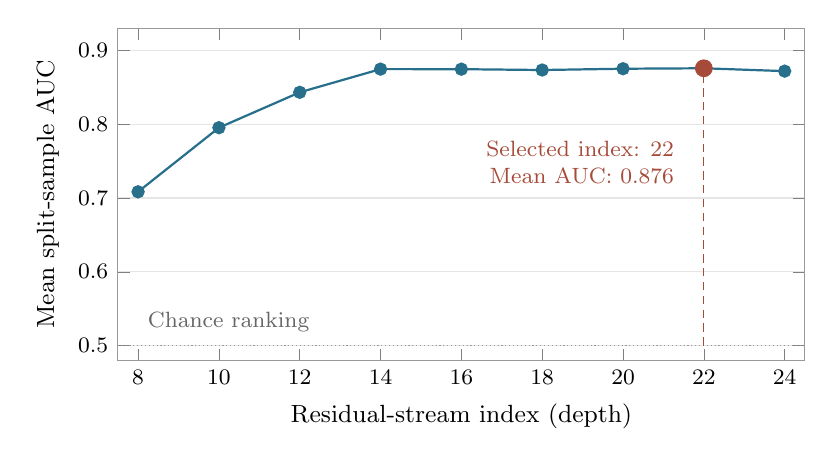
\begin{tikzpicture}
\definecolor{layerblue}{HTML}{286F8C}\definecolor{layerorange}{HTML}{A64B39}
\begin{axis}[width=.85\linewidth,height=5.8cm,xmin=7.5,xmax=24.5,ymin=.48,ymax=.93,xtick={8,10,12,14,16,18,20,22,24},ytick={.5,.6,.7,.8,.9},xlabel={Residual-stream index (depth)},ylabel={Mean split-sample AUC},label style={font=\small},tick label style={font=\footnotesize},axis line style={black!40},ymajorgrids,grid style={black!10}]
\addplot[black!40,densely dotted] coordinates {(7.5,.5)(24.5,.5)};
\addplot[thick,color=layerblue,mark=*,mark size=2pt] coordinates {(8,0.7083884479717814) (10,0.7952374790495909) (12,0.8431731790945042) (14,0.8745912616254232) (16,0.8745210846013124) (18,0.8733831898298773) (20,0.8751263186433994) (22,0.8757466150711491) (24,0.871869077743819)};
\draw[densely dashed,layerorange] (axis cs:22,.5) -- (axis cs:22,0.8757466150711491);
\addplot[only marks,mark=*,mark size=3pt,color=layerorange] coordinates {(22,0.8757466150711491)};
\node[font=\footnotesize,align=right,anchor=north east,text=layerorange] at (axis cs:21.5,.79) {Selected index: 22\\Mean AUC: 0.876};
\node[font=\footnotesize,anchor=south west,text=black!60] at (axis cs:8,.505) {Chance ranking};
\end{axis}\end{tikzpicture}
\par\medskip% The selected site feeds four exploratory questions; same samples are reused.
\begin{tikzpicture}[font=\fontsize{8.5}{10}\selectfont,
flow/.style={-{Latex[length=1.8mm]},thick,draw=black!45},
panel/.style={draw=black!20,rounded corners=2pt,fill=black!2,text width=3.0cm,align=center,inner sep=4pt,minimum height=2.4cm}]
\definecolor{pointblue}{HTML}{286F8C}
\definecolor{pointorange}{HTML}{A64B39}
\node[align=center,text width=13.6cm,font=\fontsize{10}{12}\selectfont\bfseries] (refit) at (7,0) {C. Re-estimate at index 22 on the full sample; examine MH1--MH4};
\coordinate (hub) at (7,-.55);
\draw[flow] (refit.south) -- (hub);
\node[panel,anchor=north] (one) at (1.7,-.95) {\textbf{MH\textsubscript{1}: signal}\\[3pt]Within-language AUC\\[4pt]\textcolor{pointblue}{All 21 cells above chance}};
\node[panel,anchor=north] (two) at (5.2,-.95) {\textbf{MH\textsubscript{2}: transfer}\\[3pt]Source A $\rightarrow$ target B\\[4pt]\textcolor{pointblue}{Reference and ANITA:\\higher transfer AUC}};
\node[panel,anchor=north] (three) at (8.7,-.95) {\textbf{MH\textsubscript{3}: behavior}\\[3pt]AUC / cosine\\vs. mean score\\[4pt]\textcolor{pointorange}{Mixed across models}};
\node[panel,anchor=north] (four) at (12.2,-.95) {\textbf{MH\textsubscript{4}: models}\\[3pt]Portability + addition\\[4pt]\textcolor{pointorange}{Portability differs\\Matched steering\\remains unresolved}};
\foreach \n in {one,two,three,four}{\draw[flow] (hub) -| (\n.north);}
\node[fit=(one)(two)(three)(four),inner sep=0] (checks) {};
\node[align=center,text width=13.6cm,text=black!65,font=\fontsize{8}{9.5}\selectfont] at ([yshift=-.5cm]checks.south) {Reused samples and shared question identities: these are exploratory checks, with no independent final question holdout.};
\end{tikzpicture}

\label{fig:mechanistic-layer-sweep}\fonte{Prepared by the author (2026).}\end{figure}
